\begin{comment}
Existing OpenMCT implementations

Design suggestion: Backend server in Node, which gets, parses and stores telemetry, and allows Open MCT and other users to request data in a simple and easily readable format
 - Abstracts away unknowns in connection to NA - rate limits, uptime, accessibility
 - Allows “offline” usage, load telemetry from file or other sources
 - Generate required OMCT data, servers and parsers from definition - trying to minimize code overhead for adding new data
 - Open MCT is the hard part; aim with code should be to minimize work required to get new inputs accessible in Open MCT, since it's the largest unknown
\end{comment}

\section{Design and Implementation}
\subsection{Introduction}
With an overview of the necessary inputs and outputs of the system, and the requirements placed on its functionality and performance, it is possible to develop a draft for the design and implementation. This version will be referred to as version 0, or v0 for short.

From the requirements and restrictions on access to the \Gls{nanoavionics} telemetry server, it is clear that the system will need to have local storage to store telemetry data to decouple Open MCT from this server. Giving every device that Open MCT should be available on direct access to the \Gls{nanoavionics} server is not feasible, due to the time needed to manually approve the IP address for each device and issue new authentication keys. Their server is an entity that is to some degree unknown, and does not have any specific guarantees on availability or performance. 

Since Open MCT will need to be hosted by a web server of some kind to be accessible in a web browser, implementing the required telemetry storage and parsing mechanisms on this web server would also aid with meeting the requirements for telemetry data availability outside Open MCT (see \acrshort{fr}3.0 and \acrshort{nfr}7.0) by providing it over \acrshort{http}.

\begin{figure}[H]
  \centering
  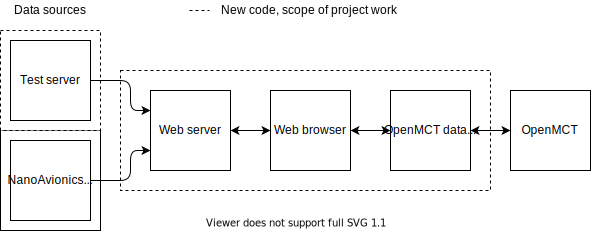
\includegraphics[width=0.75\linewidth]{Images/Diagrams/Block Diagram (early).png}
  \caption{Early system block diagram}
  \label{fig:block}
\end{figure}

A simple high-level system block diagram for such a system is shown in Figure \ref{fig:block}, showing each component and the connections between them. The test server is an alternate data source that provides similar output to the NanoAvionics server, to aid with testing and development, as the NA server may not be available at all times making an alternate telemetry data source an essential component.

\begin{figure}[H]
  \centering
  \includegraphics[width=0.8\linewidth]{Images/Diagrams/MCT Depot.png}
  \caption{MCT Depot overview}
  \label{fig:mctdepot}
\end{figure}

To make it easier to distinguish between new and existing code, the system that is to be implemented inside the dashed lines in Figure \ref{fig:block} has been given the name \emph{MCT Depot}, or just \emph{Depot} for short. The name comes from structure and function of the system resembling that of a train or bus depot, in that it processes and temporarily stores incoming telemetry data from various origins before routing it on to Open MCT or another destination, as seen in Figure \ref{fig:mctdepot}.

\subsection{Language and framework selection}
To implement \Gls{depot} as outlined above, it was as consequence of \acrshort{nfr}10.0 decided to use JavaScript (in the form of \Gls{ecma}) for the \gls{backend} since it’s already used in the Open MCT \gls{frontend}. This avoids introducing more than one new programming language for the HYPSO project to support in relation to this system, and encourages code reuse between the \gls{frontend} and \gls{backend}.

\subsection{Proposed system architecture}
Seeing as \Gls{depot} should be independent of the telemetry data source - it shouldn't matter to the destinations whether the telemetry is coming directly from \Gls{nanoavionics}’ server, a file-based backup, or another server providing some kind of relevant data - it was natural to split it into four more or less independent parts: The telemetry fetching system, the telemetry processing subsystem, the data management and storage system, and the telemetry serving system. The data management and storage system is the link between the otherwise independent telemetry fetching and telemetry serving systems.

It was decided to use \Gls{node} running an \Gls{express}-based web app to host and manage each of these subsystems. \Gls{express} was chosen since it is one of the most used and well-documented web server frameworks for \Gls{node}, and has already been used in multiple other successful implementations of Open MCT telemetry servers, including the current official Open MCT server implementation tutorial.

Based on the block diagram above a data flow diagram for the full system was created to get an idea of the types and amounts of data that would be going between each subsystem. This can be found in Figure \ref{fig:dfd}.

\begin{figure}[H]
  \centering
  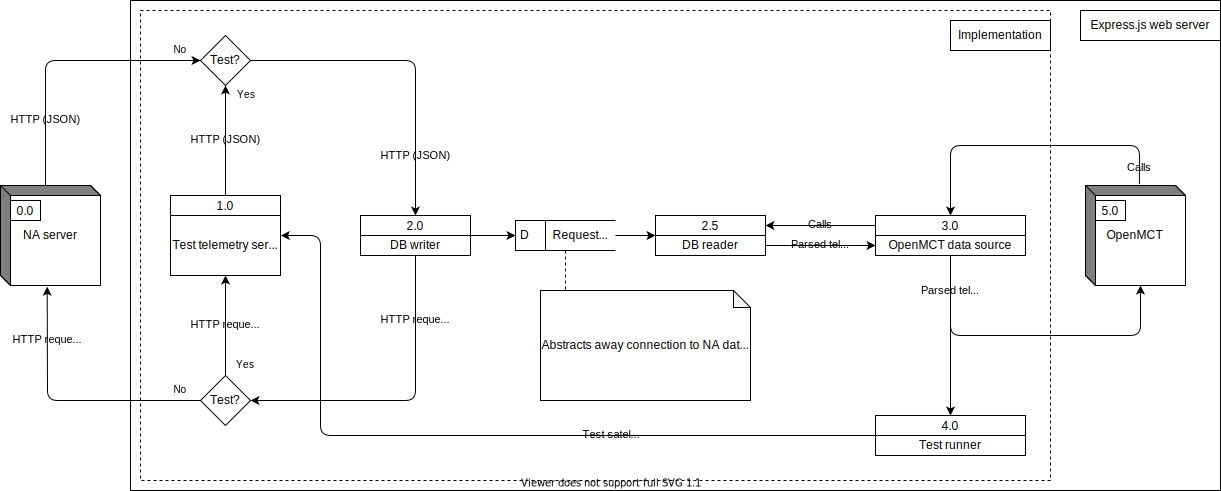
\includegraphics[width=1\linewidth]{Images/Diagrams/Data Flow Diagram (L0).png}
  \caption{v0 Level 0 Data Flow Diagram}
  \label{fig:dfd}
\end{figure}

After this a complete class diagram with the full planned extent of modules, with descriptions of their local variables and methods was created. This will be referenced actively in the section below outlining the functionality and decisions behind the implementation of each module. This can be found in Figure \ref{fig:class}, with cutouts for each subsystem found in figures \ref{fig:cdshared} to \ref{fig:cdserving}.

\begin{sidewaysfigure}[ht]
  \centering
  \includegraphics[width=1\linewidth]{Images/Diagrams/Class Diagram Large.png}
  \caption{v0 Class Diagram Overview}
  \label{fig:class}
\end{sidewaysfigure}

Attempting to read Figure \ref{fig:class} directly is not recommended, and it is mostly included as a way to get a quick overview of the connections between the subsystems.

\subsubsection{Shared modules}
These provide simple but important utility functions, such as managing the current configuration of the system and allowing it to be imported/exported to a file, plus providing a system log.

The class diagram for these modules can be found in Figure \ref{fig:cdshared}.

\begin{figure}[H]
  \centering
  \includegraphics[width=1\linewidth]{Images/Diagrams/SharedModules.png}
  \caption{v0 Class Diagram: Shared Modules}
  \label{fig:cdshared}
\end{figure}

The \inlinecode{Config} module provides a reasonable set of default settings, so that external configuration files only need to contain the settings to be changed or added if the defaults do not suit the intended use of the system.

\subsubsection{Telemetry fetching subsystem}
This subsystem provides an interface for getting telemetry data from external origins. It is implemented by the \inlinecode{TelemetryFetcher} class, which is realised for various specific external sources as \inlinecode{FileTelemetryProvider}, \inlinecode{TestTelemetryProvider}, and \inlinecode{NATelemetryProvider}. As the names imply, these get telemetry data from a file, a test spacecraft, and NanoAvionics’ server respectively.

The default implementation of all of these are simple polling services that check their sources at a regular interval to see if there is any new data; if so this data is written to the connected \inlinecode{DbManager}. A connection to a \inlinecode{TelemetryDefinition} via \inlinecode{TelemetryParser} may be required if the telemetry type, timestamp or any metadata to be stored cannot be determined directly from the received data without it being \glslink{unpacking}{unpacked} and parsed first. These modules will be introduced in the next section.

The class diagram for these modules can be found in Figure \ref{fig:cdfetching}.

\begin{figure}[H]
  \centering
  \includegraphics[width=0.7\linewidth]{Images/Diagrams/TelemetryFetching.png}
  \caption{v0 Class Diagram: Telemetry Fetching}
  \label{fig:cdfetching}
\end{figure}

\subsubsection{Telemetry processing subsystem}
The top-level module here, \inlinecode{TelemetryParser}, provides methods for configuring, parsing and \gls{unpacking} various types of telemetry data, with a general class \inlinecode{TelemetryDefinition} that has a special subclass \inlinecode{NATelemetryDefinition} that provides a quick way to set up the \inlinecode{TelemetryDefinition}s for each type of telemetry we get directly from NanoAvionics’ server.

The data that is returned from NanoAvionics’ using their \Gls{postgrest}-based \acrshort{http} API is in the form of JSON with some basic metadata and, more importantly, a string that contains a \glslink{packing}{packed} C-style \gls{struct}. In \inlinecode{NATelemetryDefinition} we use a third-party module called \gls{ezstruct} that allows us to quickly convert this to JSON based directly on the \gls{struct} header definitions we get in text files from NanoAvionics, speeding up the process of implementing and updating the telemetry definitions greatly (as required by \acrshort{nfr}6.0). Updating or adding a new \inlinecode{TelemetryDefinition} for parsing telemetry data from NanoAvionics’ should be as simple as downloading the \gls{struct} header file and updating \Gls{depot}'s configuration to include it.

The class diagram for this subsystem can be found in Figure \ref{fig:cdparsing}.

\begin{figure}[H]
  \centering
  \includegraphics[width=1\linewidth]{Images/Diagrams/TelemetryParsing.png}
  \caption{v0 Class Diagram: Telemetry Parsing}
  \label{fig:cdparsing}
\end{figure}

\subsubsection{Data management and storage subsystem}
The next major part is the \inlinecode{DbManager}, which handles storing data (usually from a \inlinecode{TelemetryFetcher}) and reading data (usually from a \inlinecode{TelemetryServer}). The interface here is fairly simple, as the proposed implementation just has a single table that can be indexed by timestamp and type (which maps to a \inlinecode{TelemetryDefinition} that can be used to \glslink{unpacking}{unpack} the data stored for that type).

%\todo[inline]{Describe suggested database schema in detail}

The class diagram for this subsystem can be found in Figure \ref{fig:cddb}.

\begin{figure}[H]
  \centering
  \includegraphics[width=0.65\linewidth]{Images/Diagrams/DbManager.png}
  \caption{v0 Class Diagram: Database Management}
  \label{fig:cddb}
\end{figure}

To host the database it was decided to use SQLite; the fairly simple structure of the database used works well with it, and the large benefits it provides in portability (for \say{offline} work or quick backups) due to the database being stored in a single file made it a good candidate compared to other more complex database solutions.

Using some kind of object-relational mapping framework - such as Sequelize - was investigated but eventually dropped, due to the low level of complexity in the proposed database schema and the queries required. There was also a lack of demand for many of the features that these frameworks come with, such as support for generating database migrations to preserve data if the database schema is updated. The database functions more as a cache or buffer for processed telemetry data than a primary source of it, with new copies of the raw telemetry data being available and backed up in other locations (albeit with higher latency and request complexity until it is imported into the database again).

\subsubsection{Telemetry serving subsystem}
This subsystem hosts and manages one or more \acrshort{http}/\Gls{ws} servers for getting data for a specified \inlinecode{TelemetryDefinition} from a \inlinecode{DbManager}. The \acrshort{http} servers (implemented by \inlinecode{HistoryServer}) are used for allowing a service to request historical data for a period, while the \Gls{ws} servers (implemented by \inlinecode{RealtimeServer}) allow a service to subscribe to real-time data updates without having to continuously poll a \acrshort{http} server.

The class diagram for this subsystem can be found in Figure \ref{fig:cdserving}.

\subsubsection{Open MCT client plugins}
These allow Open MCT to get and subscribe to telemetry data from \Gls{depot} through the telemetry serving subsystem described above, and allows mapping this data to various user-defined visualisations.

The preliminary class diagram for this subsystem can be found in Figure \ref{fig:cdserving}.

\begin{figure}[H]
  \centering
  \includegraphics[width=1\linewidth]{Images/Diagrams/TelemetryServing.png}
  \caption{v0 Class Diagram: Telemetry Server and Client}
  \label{fig:cdserving}
\end{figure}

\subsection{Code standards}
It was decided to keep the code style and syntax similar to what’s already encouraged and used by the Open MCT project in their contribution guidelines \cite{omct_contributing} for both the \gls{backend} and new \gls{frontend} code. A simplified version of Open MCT’s \Gls{eslint} configuration file is used to enforce this code style throughout the project, where the simplifications are the removal of configuration specific to external dependencies not used by \Gls{depot}.